\section{Q2} 

\subsection{Introduction} \label{sec:Introduction}

In the context of industrial automation, conveyor belt systems play a crucial role in material handling processes, 
ensuring continuous and efficient movement of goods within a production line. The objective of this laboratory task 
is to design, simulate, and analyze an electromagnetic control system to manage the operation of a conveyor belt, 
driven by a single-phase AC induction motor.

The system's functional specifications demand a controlled startup delay, immediate stoppage via a stop push 
button, and an automatic halt upon the activation of a limit switch sensor. To meet these requirements, the 
control architecture integrates key components such as a general magnetic circuit breaker, a thermal relay, 
a lamp emulator, and push buttons configured with normally open (NO) and normally closed (NC) contacts.

This report outlines the design process, starting with the development of a Grafcet diagram representing the 
sequence of operations, followed by the assembly diagram detailing the connections between components. From this, 
both the electrical power and command circuits are derived. Finally, the proposed system is simulated using 
Fluidsim 3.6 to verify that it meets the operational specifications. Through this exercise, essential concepts 
of electromagnetic technology applied to industrial control systems are reinforced, with emphasis on safety, 
responsiveness, and process reliability.

\subsection{Process Schematic and Sensor-Actuator Integration} \label{sec:Process_Schematic_and_Sensor-Actuator_Integration}

The first step in the system design is to create a eletrical circuit representation of the process, 
illustrating the placement of sensors and actuators. This diagram serves as a foundational blueprint 
for the entire control system. The schematic includes the necessary cylinders, valves, and control 
components to facilitate automation.

\begin{figure}[H]
    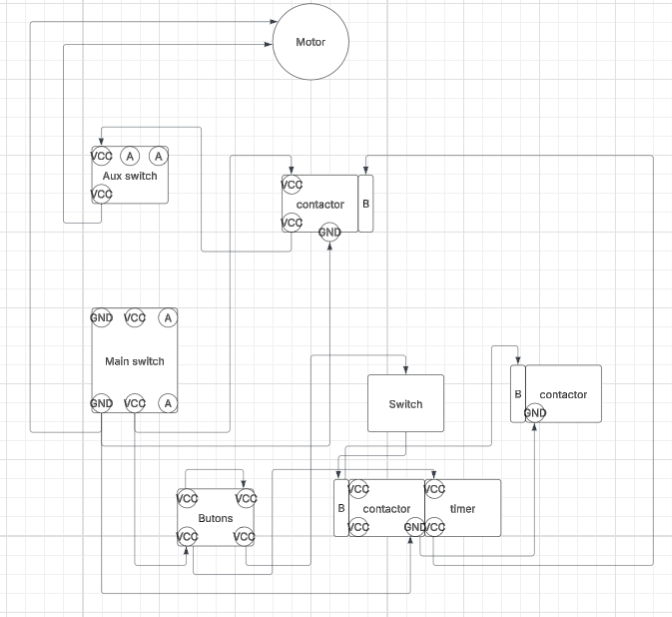
\includegraphics[width=16cm]{Images/Q2/eletrical_circuit.png}
    \centering
    \caption{Decided schematic for the door control}
    \label{fig:eletrical_circuit}
\end{figure}


This schematic\ref{fig:eletrical_circuit} illustrates the design of a double-cylinder door mechanism. Both Buttons B1 and B2 
can be used to open the door, which remains open for approximately five seconds after the button is 
released. Additionally, two emergency buttons (B3 and B0) are included—one pneumatic and the other 
electropneumatic—to disconnect the compressor in case of an emergency.

\subsection{Grafcet Representation} \label{sec:Grafcet_Representation}

A structured graphical representation of the automation sequence is developed using the 
Grafcet method. This step-by-step graphical model illustrates the transitions between 
different states of the system, ensuring a clear understanding of the control logic.

This first model is a simple user view of the grafset

\begin{figure}[H]
    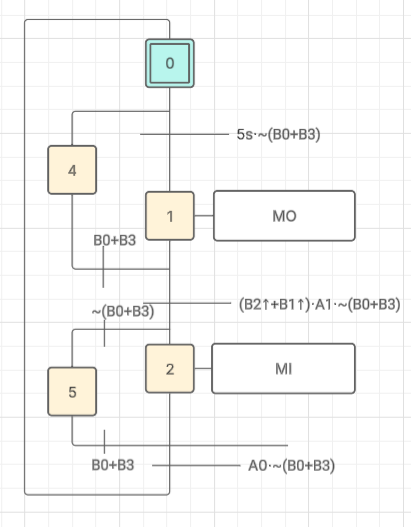
\includegraphics[width=16cm]{Images/Q2/grafset_simple.png}
    \centering
    \caption{Grafset for the door control}
    \label{fig:grafset_simple}
\end{figure}

The second model is a more complex grafset representing the real actuators/contactos mechanism

\begin{figure}[H]
    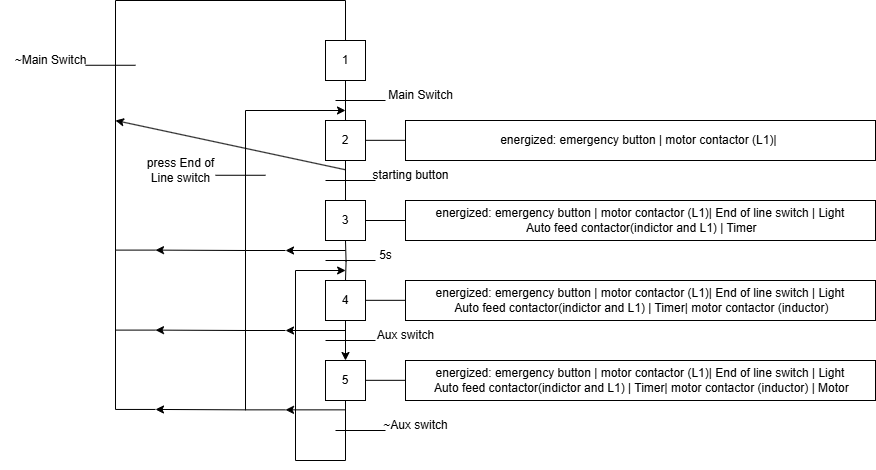
\includegraphics[width=16cm]{Images/Q2/grafset_complex.png}
    \centering
    \caption{Grafset for the door control}
    \label{fig:grafset_complex}
\end{figure}

\subsection{Simulation and Validation} \label{sec:Simulation_and_Validation}

The final stage involves simulating the closed-loop control system in Fluidism 3.6 software. 
The simulation tests the interaction between the automation process, sensors, and actuators, 
validating whether the system meets the defined specifications. Any deviations are analyzed, 
and necessary modifications are proposed to optimize system performance.

\begin{figure}[H]
    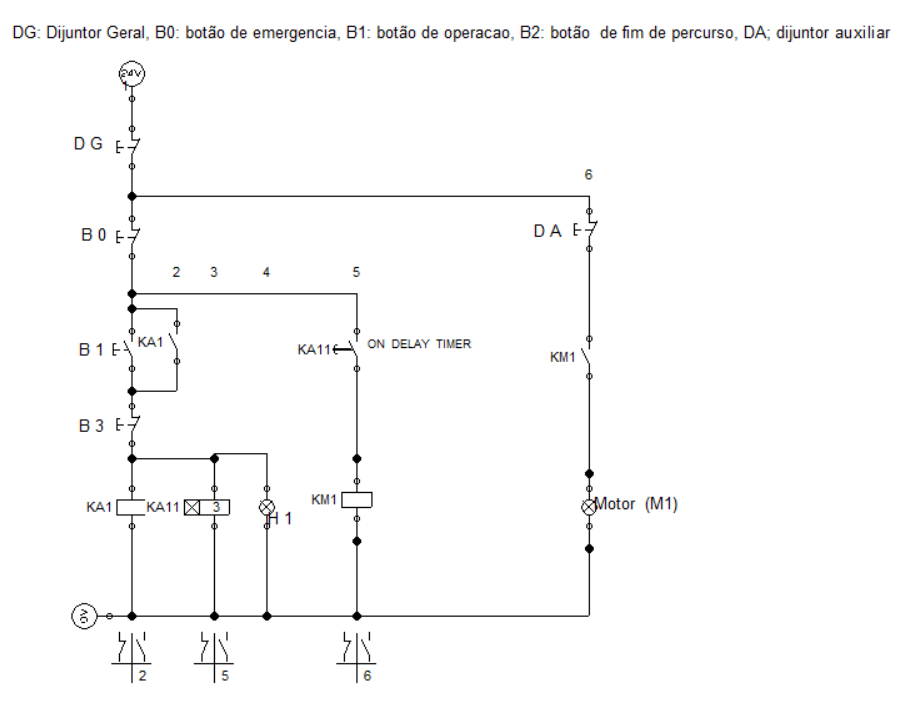
\includegraphics[width=16cm]{Images/Q2/fluidsim.png}
    \centering
    \caption{Fluidsim for the motor control}
    \label{fig:fluidsim}
\end{figure}

The complete implementation of the control system in FluidSim 3.6 is shown here. The design includes two OR gates, 
allowing both control buttons to be used as needed. The emergency buttons (one pneumatic and one electropneumatic) 
are also visible. Due to software constraints, the circuit controlling the light and buzzer had to be duplicated, as 
each pneumatic-to-electrical converter could only be connected to a single differential pressure switch—one for the 
opening motion and another for closing.\\

\subsection{Conclusion}

This report details the complete development of an electropneumatic control system, from schematic 
design to simulation validation. By integrating various automation components and methodologies, 
the system achieves a robust and efficient control mechanism. The findings highlight the importance 
of precise component selection and control logic design in achieving a functional and reliable 
automated process.